%Amazon


\begin{figure}[H]
\centering
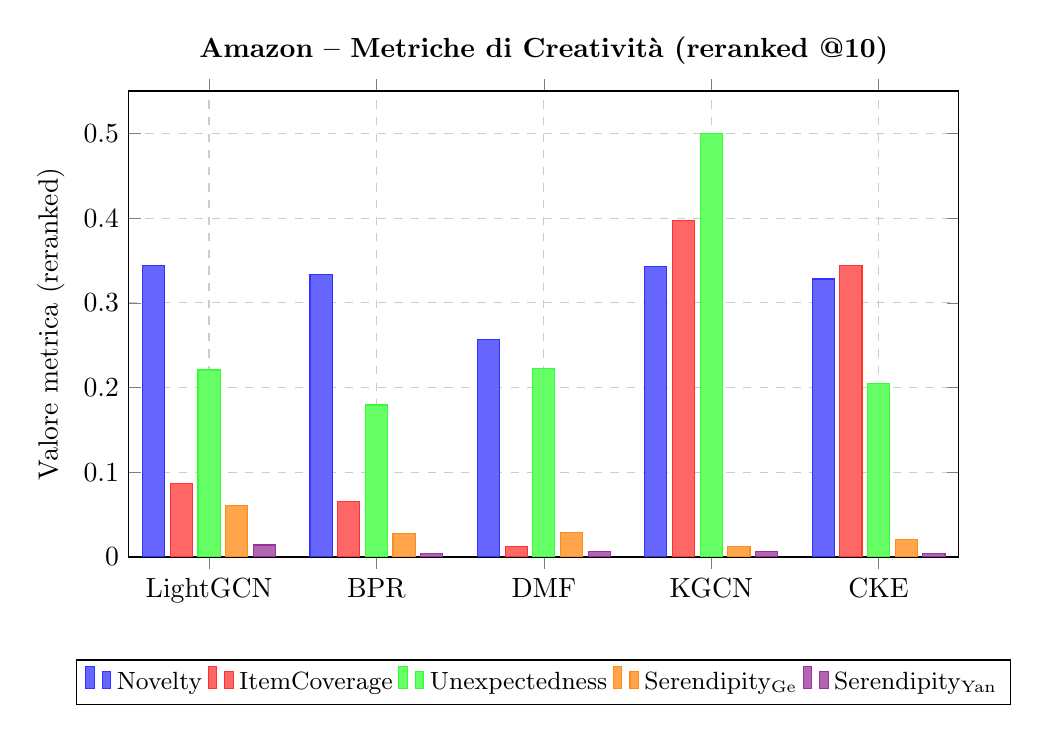
\begin{tikzpicture}
\begin{axis}[
    ybar,
    bar width=8pt,
    width=\textwidth,
    height=7.5cm,
    enlarge x limits=0.12,
    legend style={at={(0.5,-0.22)}, anchor=north, legend columns=5, font=\small},
    ylabel={Valore metrica (reranked)},
    symbolic x coords={LightGCN, BPR, DMF, KGCN, CKE},
    xtick=data,
    ymin=0,
    title={Amazon -- Metriche di Creatività (reranked @10)},
    title style={font=\bfseries},
    grid=major,
    grid style={dashed, gray!40},
]
\addplot[fill=blue!60, draw=blue!80]
    coordinates {(LightGCN,0.3439) (BPR,0.3331) (DMF,0.2566) (KGCN,0.3431) (CKE,0.3282)};
\addplot[fill=red!60, draw=red!80]
    coordinates {(LightGCN,0.0868) (BPR,0.0653) (DMF,0.0125) (KGCN,0.3974) (CKE,0.3442)};
\addplot[fill=green!60, draw=green!80]
    coordinates {(LightGCN,0.2208) (BPR,0.1794) (DMF,0.2228) (KGCN,0.5002) (CKE,0.2049)};
\addplot[fill=orange!70, draw=orange!90]
    coordinates {(LightGCN,0.0603) (BPR,0.0280) (DMF,0.0285) (KGCN,0.0127) (CKE,0.0201)};
\addplot[fill=violet!60, draw=violet!80]
    coordinates {(LightGCN,0.0141) (BPR,0.0045) (DMF,0.0060) (KGCN,0.0067) (CKE,0.0040)};
\legend{Novelty, ItemCoverage, Unexpectedness,
        Serendipity\textsubscript{Ge}, Serendipity\textsubscript{Yan}}
\end{axis}
\end{tikzpicture}
\caption{Confronto delle metriche di creatività reranked @10 sui cinque modelli (Amazon)}
\label{fig:rq1_amazon}
\end{figure}








%MovieLens


\begin{figure}[H]
\centering
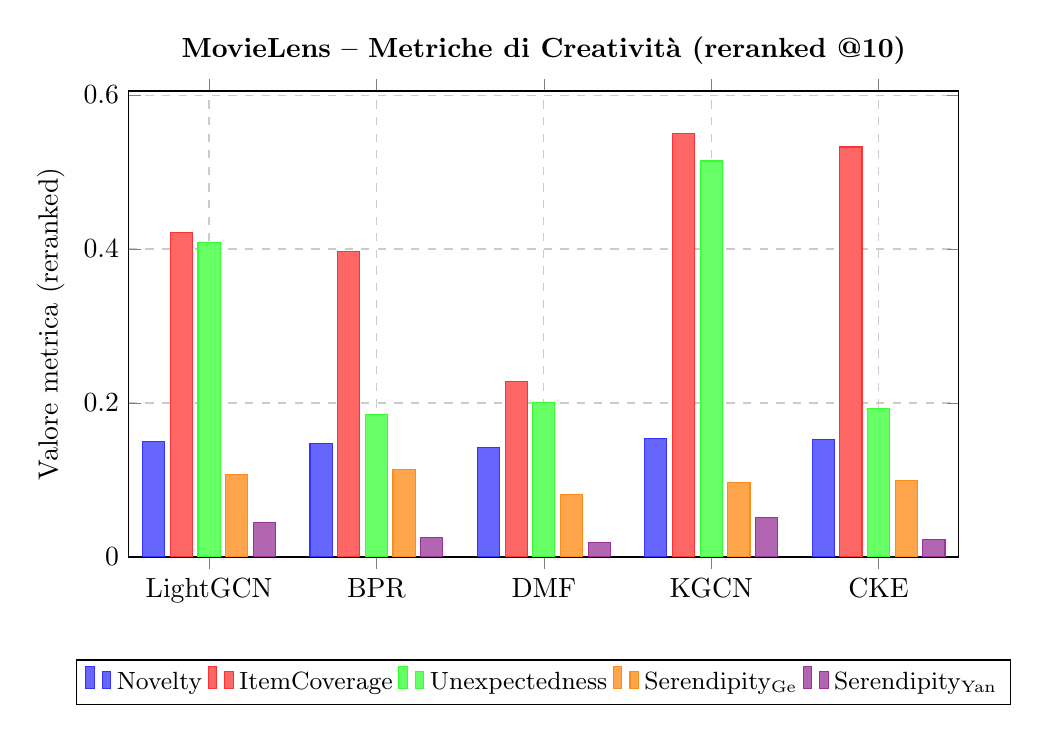
\begin{tikzpicture}
\begin{axis}[
    ybar,
    bar width=8pt,
    width=\textwidth,
    height=7.5cm,
    enlarge x limits=0.12,
    legend style={at={(0.5,-0.22)}, anchor=north, legend columns=5, font=\small},
    ylabel={Valore metrica (reranked)},
    symbolic x coords={LightGCN, BPR, DMF, KGCN, CKE},
    xtick=data,
    ymin=0,
    title={MovieLens -- Metriche di Creatività (reranked @10)},
    title style={font=\bfseries},
    grid=major,
    grid style={dashed, gray!40},
]
\addplot[fill=blue!60, draw=blue!80]
    coordinates {(LightGCN,0.1503) (BPR,0.1479) (DMF,0.1426) (KGCN,0.1543) (CKE,0.1531)};
\addplot[fill=red!60, draw=red!80]
    coordinates {(LightGCN,0.4216) (BPR,0.3968) (DMF,0.2285) (KGCN,0.5503) (CKE,0.5325)};
\addplot[fill=green!60, draw=green!80]
    coordinates {(LightGCN,0.4082) (BPR,0.1854) (DMF,0.2007) (KGCN,0.5143) (CKE,0.1931)};
\addplot[fill=orange!70, draw=orange!90]
    coordinates {(LightGCN,0.1070) (BPR,0.1132) (DMF,0.0813) (KGCN,0.0968) (CKE,0.0992)};
\addplot[fill=violet!60, draw=violet!80]
    coordinates {(LightGCN,0.0450) (BPR,0.0251) (DMF,0.0186) (KGCN,0.0511) (CKE,0.0226)};
\legend{Novelty, ItemCoverage, Unexpectedness,
        Serendipity\textsubscript{Ge}, Serendipity\textsubscript{Yan}}
\end{axis}
\end{tikzpicture}
\caption{Confronto delle metriche di creatività reranked @10 sui cinque modelli (MovieLens)}
\label{fig:rq1_movielens}
\end{figure}